\chapter{Designs \& Architecture} \label{appendix_designs} 

\section{Component Layer Naming Conventions} \label{appendix_component_naming_convention}

\textbf{[\gls{prod}]} is defined as \textit{\glsdesc{prod}} \newline 
\textbf{[\gls{comp}]} is defined as \textit{\glsdesc{comp}} \newline 
\textbf{[\gls{tech}]} is defined as \textit{\glsdesc{tech}} 

\begin{table}[H]
    \footnotesize
    \begin{tabular}{ l p{0.30\linewidth} p{0.43\linewidth} }
    \hline
    \textbf{Layer} & \textbf{Project name} & \textbf{Package name} \\ 
    \hline
    Domain & [\gls{prod}].Domain & [\gls{comp}].[\gls{prod}].Domain \\
    Application & [\gls{prod}].Application & [\gls{comp}].[\gls{prod}].Application \\
    Presentation & [\gls{prod}].Presentation.[\gls{tech}] & [\gls{comp}].[\gls{prod}].Presentation.[\gls{tech}] \\
    Infrastructure & [\gls{prod}].Infrastructure.[\gls{tech}] & [\gls{comp}].[\gls{prod}].Infrastructure.[\gls{tech}]
    \\ \hline
    \end{tabular}
\caption{Naming convention component layers}
\label{table:component_naming_convention}
\end{table}

\section{Element Naming Conventions} \label{appendix_element_naming_convention}

\textbf{[\gls{verb}]} is defined as \textit{\glsdesc{verb}} \newline 
\textbf{[\gls{noun}]} is defined as \textit{\glsdesc{noun}} 

\begin{table}[H]
  \footnotesize
  \begin{tabular}{ l p{0.24\linewidth} p{0.09\linewidth} p{0.37\linewidth} }
  \hline
  \textbf{Layer name} & \textbf{Element} & \textbf{Type} & \textbf{Naming Convention} \\ \hline
  Presentation & Controller & class & [\textit{\gls{noun}}]Controller \\
  & ViewModelMapper & class & [\textit{\gls{noun}}]ViewModelMapper \\
  & Presenter & class & [\textit{\gls{verb}}][\textit{\gls{noun}}]Presenter \\
  & ViewModel & class & [\textit{\gls{noun}}]ViewModel \\

  Application & Boundary & class & [\textit{\gls{verb}\gls{noun}}]Boundary \\
  & Boundary  & interface & IBoundary \\
  & Gateway  & interface & I[\textit{\gls{verb}}]Gateway \\
  & Interactor  & interface & I[\textit{\gls{verb}}]Interactor \\
  & Interactor & class & [\textit{\gls{verb}}][\textit{\gls{noun}}]Interactor \\
  & Mapper  & interface & IMapper \\
  & RequestModelMapper & class & [\textit{\gls{verb}}][\textit{\gls{noun}}]RequestModelMapper \\
  & Presenter  & interface & IPresenter \\
  & Validator  & interface & IValidator \\
  & Validator & class & [\textit{\gls{verb}}][\textit{\gls{noun}}]Validator \\
  
  Infrastructure & Gateway & class & [\textit{\gls{noun}}]Repository \\

  Domain & Data Entity & class & [\textit{\gls{noun}}] \\ \hline

  \end{tabular}
  \caption{Naming convention of recurring elements}
  \label{table_element_naming_convention}
\end{table}

\section{UML2 Notation Legenda} \label{appendix_legenda} 

In order to visualize the designs of the artifact, a standard UML notation is used. The
designs containing relationships adhere to the following definitions.

\begin{figure}[H]
  \centering
  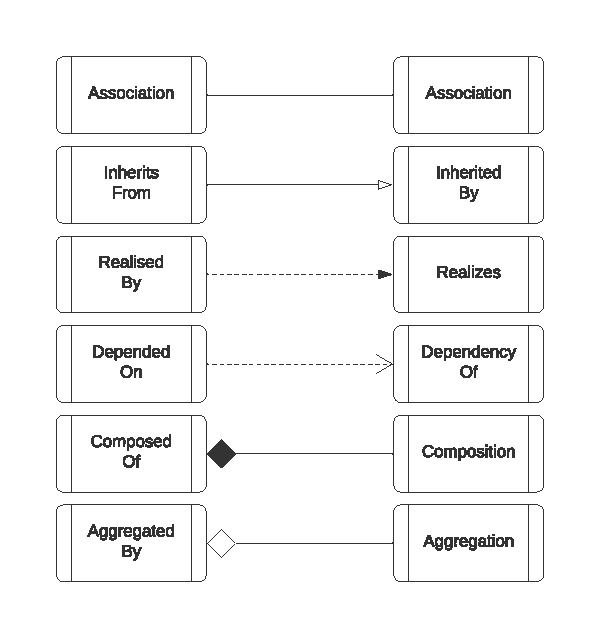
\includegraphics[width=0.5\textwidth]{figures/class_diagram_legenda.pdf}
  \caption[UML Notation used]{UML notation}
  \label{fi:class_diagram_relationship_notation}
\end{figure}